% A LaTeX (non-official) template for ISAE projects reports
% Copyright (C) 2014 Damien Roque
% Version: 0.2
% Author: Damien Roque <damien.roque_AT_isae.fr>

\documentclass[a4paper,12pt]{book}
\usepackage[utf8]{inputenc}             % The input file is in utf-8
\usepackage{marvosym}                   % This package provides some symbols. The € is 
\DeclareUnicodeCharacter{20AC}{\EUR{}} 
\usepackage[utf8]{inputenc}
\usepackage[T1]{fontenc}
\usepackage[frenchb]{babel} % If you write in French
%\usepackage[english]{babel} % If you write in English
\usepackage{a4wide}
\usepackage{graphicx}
\graphicspath{{images/}}
\usepackage{subfig}
\usepackage{tikz}
\usepackage{float} 
\usetikzlibrary{shapes,arrows}
\usepackage{pgfplots}
\pgfplotsset{compat=newest}
\pgfplotsset{plot coordinates/math parser=false}
\newlength\figureheight
\newlength\figurewidth
\pgfkeys{/pgf/number format/.cd,
set decimal separator={,\!},
1000 sep={\,},
}
\usepackage{ifthen}
\usepackage{ifpdf}
\ifpdf
\usepackage[pdftex]{hyperref}
\else
\usepackage{hyperref}
\fi
\usepackage{color}
\hypersetup{%
colorlinks=true,
linkcolor=black,
citecolor=black,
urlcolor=black}

\renewcommand{\baselinestretch}{1.05}
\usepackage{fancyhdr}
\pagestyle{fancy}
\fancyfoot{}
\fancyhead[LE,RO]{\bfseries\thepage}
\fancyhead[RE]{\bfseries\nouppercase{\leftmark}}
\fancyhead[LO]{\bfseries\nouppercase{\rightmark}}
\setlength{\headheight}{15pt}

\let\headruleORIG\headrule
\renewcommand{\headrule}{\color{black} \headruleORIG}
\renewcommand{\headrulewidth}{1.0pt}
\usepackage{colortbl}
\arrayrulecolor{black}

\fancypagestyle{plain}{
  \fancyhead{}
  \fancyfoot[C]{\thepage}
  \renewcommand{\headrulewidth}{0pt}
}

\makeatletter
\def\@textbottom{\vskip \z@ \@plus 1pt}
\let\@texttop\relax
\makeatother

\makeatletter
\def\cleardoublepage{\clearpage\if@twoside \ifodd\c@page\else%
  \hbox{}%
  \thispagestyle{empty}%
  \newpage%
  \if@twocolumn\hbox{}\newpage\fi\fi\fi}
\makeatother

\usepackage{amsthm}
\usepackage{amssymb,amsmath,bbm}
\usepackage{array}
\usepackage{bm}
\usepackage{multirow}
\usepackage[footnote]{acronym}

\newcommand*{\SET}[1]  {\ensuremath{\mathbf{#1}}}
\newcommand*{\VEC}[1]  {\ensuremath{\boldsymbol{#1}}}
\newcommand*{\FAM}[1]  {\ensuremath{\boldsymbol{#1}}}
\newcommand*{\MAT}[1]  {\ensuremath{\boldsymbol{#1}}}
\newcommand*{\OP}[1]  {\ensuremath{\mathrm{#1}}}
\newcommand*{\NORM}[1]  {\ensuremath{\left\|#1\right\|}}
\newcommand*{\DPR}[2]  {\ensuremath{\left \langle #1,#2 \right \rangle}}
\newcommand*{\calbf}[1]  {\ensuremath{\boldsymbol{\mathcal{#1}}}}
\newcommand*{\shift}[1]  {\ensuremath{\boldsymbol{#1}}}

\newcommand{\eqdef}{\stackrel{\mathrm{def}}{=}}
\newcommand{\argmax}{\operatornamewithlimits{argmax}}
\newcommand{\argmin}{\operatornamewithlimits{argmin}}
\newcommand{\ud}{\, \mathrm{d}}
\newcommand{\vect}{\text{Vect}}
\newcommand{\sinc}{\ensuremath{\mathrm{sinc}}}
\newcommand{\esp}{\ensuremath{\mathbb{E}}}
\newcommand{\hilbert}{\ensuremath{\mathcal{H}}}
\newcommand{\fourier}{\ensuremath{\mathcal{F}}}
\newcommand{\sgn}{\text{sgn}}
\newcommand{\intTT}{\int_{-T}^{T}}
\newcommand{\intT}{\int_{-\frac{T}{2}}^{\frac{T}{2}}}
\newcommand{\intinf}{\int_{-\infty}^{+\infty}}
\newcommand{\Sh}{\ensuremath{\boldsymbol{S}}}
\newcommand{\C}{\SET{C}}
\newcommand{\R}{\SET{R}}
\newcommand{\Z}{\SET{Z}}
\newcommand{\N}{\SET{N}}
\newcommand{\K}{\SET{K}}
\newcommand{\reel}{\mathcal{R}}
\newcommand{\imag}{\mathcal{I}}
\newcommand{\cmnr}{c_{m,n}^\reel}
\newcommand{\cmni}{c_{m,n}^\imag}
\newcommand{\cnr}{c_{n}^\reel}
\newcommand{\cni}{c_{n}^\imag}
\newcommand{\tproto}{g}
\newcommand{\rproto}{\check{g}}
\newcommand{\LR}{\mathcal{L}_2(\SET{R})}
\newcommand{\LZ}{\ell_2(\SET{Z})}
\newcommand{\LZI}[1]{\ell_2(\SET{#1})}
\newcommand{\LZZ}{\ell_2(\SET{Z}^2)}
\newcommand{\diag}{\operatorname{diag}}
\newcommand{\noise}{z}
\newcommand{\Noise}{Z}
\newcommand{\filtnoise}{\zeta}
\newcommand{\tp}{g}
\newcommand{\rp}{\check{g}}
\newcommand{\TP}{G}
\newcommand{\RP}{\check{G}}
\newcommand{\dmin}{d_{\mathrm{min}}}
\newcommand{\Dmin}{D_{\mathrm{min}}}
\newcommand{\Image}{\ensuremath{\text{Im}}}
\newcommand{\Span}{\ensuremath{\text{Span}}}

\newtheoremstyle{break}
  {11pt}{11pt}%
  {\itshape}{}%
  {\bfseries}{}%
  {\newline}{}%
\theoremstyle{break}

%\theoremstyle{definition}
\newtheorem{definition}{Définition}[chapter]

%\theoremstyle{definition}
\newtheorem{theoreme}{Théorème}[chapter]

%\theoremstyle{remark}
\newtheorem{remarque}{Remarque}[chapter]

%\theoremstyle{plain}
\newtheorem{propriete}{Propriété}[chapter]
\newtheorem{exemple}{Exemple}[chapter]

\parskip=5pt
%\sloppy

\begin{document}
\let\cleardoublepage\clearpage
%%%%%%%%%%%%%%%%%%
%%% First page %%%
%%%%%%%%%%%%%%%%%%


\begin{titlepage}
\begin{center}

\includegraphics[width=0.25\textwidth]{images/universite}
\vfill

{\large Université de Paris Ouest Nanterre La Défense}\\[0.5cm]

{\large Rapport du Stage}\\[0.5cm]



% Title
\rule{\linewidth}{0.5mm} \\[0.4cm]
{ \huge \bfseries Développement de l’application Android KoopT \\[0.4cm] }
\rule{\linewidth}{0.5mm} \\[1.5cm]


\includegraphics[width=0.3\textwidth]{logo_koopt.png}\\[1cm]
\vfill
\vfill
\vfill

% Author and supervisor
\noindent
\begin{minipage}{0.7\textwidth}
  \large
    \emph{Réalisé par :}\\
- Nadia \textsc{MASLOUHI}\\
\end{minipage}%
\begin{minipage}{0.5\textwidth}
   \large
    \emph{Encadrants :} \\
- M.~Lilian \textsc{PRUD'HOMME}\\
- Mme.~Castillo Marta \textsc{RUKOZ}
\end{minipage}

\vfill
\vfill
\vfill
\vfill
\vfill
\vfill
% Bottom of the page
{\large Stage effectué du 3 Avril 2017 au 31 juillet 2017 
au sein de l'entreprise GlooKal
\vfill
\vfill
 26 juin 2017}

\end{center}
\end{titlepage}
\clearpage

\chapter*{Remerciements}
Je tiens à remercier toutes les personnes qui ont contribué au succès de mon stage et qui m’ont aidée lors de la rédaction de ce rapport. 
 
Tout d’abord, j’adresse mes remerciements à M.Philippe GAUTIER dirigeant de l’entreprise GLooKal de m’avoir accueilli comme stagiaire au sein de son entreprise.
 
Je tiens à remercier vivement M.Lilian PRUD’HOMME, mon maître de stage qui m’a formée et accompagnée tout au long de cette expérience professionnelle avec beaucoup de patience et de pédagogie. 
 
Je remercie également Mme Castillo Marta RUKOZ mon encadrante pédagogique pour son suivi tout au long de la période de stage.		
					
Enfin, j’adresse mes plus sincères remerciements à ma famille et mes amis qui m’ont soutenue et m’ont encouragée pendant cette période du stage.
\tableofcontents
\listoffigures


%%%%%%%%%%%%%%%%%%%%%%%%%%%%%%%%%%%%%%%%%%%%
%%% Content of the report and references %%%
%%%%%%%%%%%%%%%%%%%%%%%%%%%%%%%%%%%%%%%%%%%%

\mainmatter
\pagestyle{fancy}



\chapter*{Introduction}
\label{chap:introduction}
%\minitoc

84\% des français surfent quasiment quotidiennement sur leur smartphone, et ont au moins créé un rendez-vous sur un agenda électronique ; 71\% des français ont déjà utilisé leur mobile pour chercher des informations, avant d’acheter ou d’avoir recours à une prestation de service; 9 Français sur 10 ont déjà eu recours à une application dite de consommation collaborative.

En observant ces statistiques, on constate qu’un utilisateur a un besoin universel et trivial c’est de planifier, trouver, réserver rapidement et facilement des RDV avec quiconque, quel que soit le contexte, personnel ou professionnel.


L’application KOOPT s’inscrit dans le récent développement des conciergeries digitales et collaboratives, ainsi que des services de prise de rendez-vous. Pour toutes ces solutions, la promesse utilisateur est : efficacité, gain de temps, exhaustivité de l’offre, économies d’échelle et financières. Toutefois, ces outils, essentiellement basés sur des plateformes d’échange centralisées, rencontrent de nombreux freins à l’adoption massive : la sectorisation (verticalisation de l’offre), le manque d’automatisation (planification d’un même RDV pour plusieurs participants), l’adaptabilité et la flexibilité (gestion des aléas ou des contraintes en temps réel et de façon simultanée/parallèle), la communication ad hoc entre les acteurs... ou encore la confidentialité des échanges ou des données personnelles. 
				
Dans le cadre de ma première année de Master MIAGE (Méthodes informatiques appliquées à la gestion des entreprise) à l'Université de Paris ouest Nanterre la Défense, j'ai souhaité réaliser mon stage dans une entreprise répondant à ces enjeux par une application mobile Android tout en me formant sur le développement des applications Android (Programmation Mobile)  que ma formation propose comme débouché. 					
J'ai donc effectué un stage du 3 Avril au 31 juillet au sein de la société GLOOKAL dont l'activité est la conception et la création de l’application KOOPT. 
				
L'entreprise française GLOOKAL, créée très récemment en 2016 a pu étudier et mettre en place un tout nouveau concept (B-ADSc) pour la conception de l’application KOOPT qui se base sur l’intelligence artificielle. j'ai voulu intégrer l’équipe technique de GLOOKAL pour pouvoir découvrir les bases de ce concept ainsi de m’approfondir et m'enrichir dans la programmation des applications Android. 
 
C’est dans cette optique que s’inscrit mon projet de Master 1 et le présent rapport présente les fondements théoriques et les aspects techniques nécessaires à l’implémentation de la  nouvelle solution KOOPT.
		
Ce présent rapport est divisé en 7 chapitres :
 
Chapitre 1 : Cadre général de stage, présente l’organisme d’accueil ainsi que  le cadre général du stage.
\newline
Chapitre 2 : État de l’art, présente les différentes notions et technologies nécessaires pour le développement de KOOPT.
\newline
Chapitre 3 : Étude préalable de projet et implémentation, présente l’application KOOPT et ses objectifs.
\newline
Chapitre 4 : Planification et gestion de projet, présente les outils utilisés pour la planification et la gestion du projet.
\newline
Chapitre 5 : Compatibilité sous Android, présente la mission de gestion de compatibilité de KOOPT sur toutes les versions Android.
\newline
Chapitre 6 : Amélioration technique de KOOPT, présente les  différents améliorations de KOOPT durant le stage. 
\newline
Chapitre 7 : Débogage du Moteur KOOPT, présente la mission de débogage du KOOPT à travers les Logs.

\addcontentsline{toc}{chapter}{Introduction.}

%%% Local Variables: 
%%% mode: latex
%%% TeX-master: "isae-report-template"
%%% End: 

\chapter{Cadre général de stage}
\label{chap:Cadre general de stage}

\section*{Introduction}

Le premier chapitre de ce rapport donne un aperçu général sur l’organisme d’accueil ainsi que sur l’équipe du projet au sein de l’entreprise et décrit le context général du stage et ses objectifs.

\addcontentsline{toc}{section}{Introduction.}

\section{Présentation de GLOOKAL}

GLOOKAL SAS, créée en octobre 2016 par 5 associés fondateurs, développe une solution d'intelligence Décisionnelle Artificielle, embarquée dans une App mobile à destination des segments B2B, B2C et C2C. KOOPT est le 1er smart-assistant ‘BYOD’, 100\% intelligent, automatique, collaboratif et transparent. Personnel, il est embarqué sur chaque smartphone. Fonctionnant en pair-à-pair, c’est la première App d’intermédiation extensible à l’infini, qui ne partage aucune information personnelle et respecte réellement la vie privée de ses utilisateurs. 
À l’heure actuelle, le capital actuel (81.400,00 €) est détenu à 93,32\% par les associés fondateurs, le reste étant détenu par des investisseurs de type LOVE MONEY. GLOOKAL déjà développé un premier MVP (Produit Minimum Viable), sous Android, qui permet de tester le marché et la solution.
 \begin{itemize}
     \item Raison sociale : GLOOKAL SAS 
     \item Date de création : 26/10/2016
     \item Effectif : 2
     \item SIREN : 823 374 780
     \item Secteur d’activité : Numérique
     \item Adresse : 88 Avenue des ternes 75017 PARIS 
 \end{itemize}


\section{Business Model}
 \begin{itemize}
     \item Modèle projet (court-terme) : Implémentation ‘sur mesure’ de KOOPT pour répondre aux usages privés des entreprises (marque blanche). Ces projets permettront de garantir une traction et de générer, sur le court terme, du chiffre d’affaires. Rémunération forfaitaire et adaptée selon le profil du projet.
     \item Modèle Freemium (moyen-terme) : KOOPT sera disponible gratuitement pour le marché du grand-public (C2C), et en parallèle une version premium sera proposée aux offreurs de services professionnels pour un montant annuel de 99€ HT avec des fonctionnalités avancées.		
     \item Modèle redistributif (long-terme) : lorsqu’un professionnel sera recommandé par un utilisateur de KOOPT (agissant comme intermédiaire), une commission de 1 € sera prélevée sur ses honoraires et répartie entre GLOOKAL et l’intermédiaire. 
 \end{itemize}
		



 \section{Equipe de projet}
 
  \begin{itemize}
      \item Philippe Gautier – Président (Associé) : Provisoirement en charge du Marketing et Commercial. Travaille à temps plein sur le projet. Ex-DSI dans différentes entreprises, entrepreneur et expert sur l’Internet des Objets (depuis 2003) et les systèmes à intelligence décisionnelle distribuée.							
      \item Lilian Prud’homme - Directeur Technique (Associé) : Travaille à temps plein sur le projet. Ex-DSI et expert en Intelligence Artificielle. Ses compétences sont, le management d’équipes, le développement logiciel et les technologies SOA, ESB TALEND, ETL, ESB, MDM, BIGDATA, JAVA et Android STUDIO.
 
      \item Delphine Pautrat - Directrice Administrative et financière (Associée) : Travaille à temps partiel sur le projet. Manager expérimentée dans la finance, la comptabilité, la conduite des opérations et la gestion du changement (notamment dans l’industrie Informatique).
      \item Sid Ali ABID , stagiaire en informatique,
      \item Moi-même, Nadia MASLOUHI, stagiaire en informatique.
    
  \end{itemize}
	
							
Mon tuteur en entreprise pendant ce stage est M.Lilian PRUD’HOMME, Toutes les  étapes de développement de l’application seront validées par lui. Mes choix technologiques quant à eux, sont soumis à l’approbation de mon tuteur de stage en entreprise.

 \section{Présentation du stage}

Il s’agit d’un stage de 4 mois (du 3 Avril au 31 juillet ) qui entre dans le cadre de la première année de Master MIAGE (Méthodes informatiques appliquées à la gestion des entreprise) à l'Université de Paris ouest Nanterre la Défense, et consiste à contribuer aux évolutions de l’application KOOPT sous Android.

\subsection{Objectif de stage}

L’objectif de stage est de participer à l’évolution corrective et fonctionnelle de la version KOOPT bêta 0.8 - 0.9 en utilisant toutes les connaissances soit en programmation soit en conception et gestion de projet d’un côté et de pouvoir les améliorer et concevoir de nouvelle technologie et de nouveaux concepts d’un autre côté.
 
les différents buts du stage : 

 \begin{itemize}
     \item La compréhension du concept B-ADSc
     \item La compréhension de l’architecture de KOOPT
     \item Le développement des sous fonctionnalités de KOOPT 
     \item Débogage de l’application KOOPT
 \end{itemize}



%%% Local Variables: 
%%% mode: latex
%%% TeX-master: "isae-report-template"
%%% End: 
\chapter{Etat de l'art}
\label{sec:etat de l'art}

\section*{Introduction}

Pour mettre en place l’application KOOPT, il était nécessaire d’utiliser un large spectre de notions et de technologies. KOOPT a été développé sous Android Studio en utilisant différents outils Android, ainsi que KOOPT utilise des Web Services (REST), ainsi que Crashlytics Fabric et les Logs pour faciliter le débogage de l’application.
\addcontentsline{toc}{section}{Introduction.}



\section{L’environnement logiciel}
\subsection{Android}
\subsubsection{Présentation d’android}
Android est la plate-forme mobile la plus populaire au monde.Avec des centaines de millions d'appareils mobiles dans plus de 190 pays à travers le monde Android est la plus grande base installée de toute plate-forme mobile, chaque jour un million d’utilisateurs Android découvre cette plateforme pour la première fois et commence à chercher des applications, des jeux et d'autres contenus numériques.
Android donne une plate-forme open source de classe mondiale pour créer des applications et des jeux pour les utilisateurs Android partout, ainsi qu'un marché ouvert pour les distribuer instantanément.

\subsubsection{Architecture d’Android}


Comme le montre le schéma ci-dessous, la plateforme Android est basée sur 5 couches :
- un noyau linux.  qui fournit les drivers nécessaires 
- un ensemble d’API C/C++ fournissant des fonctionnalités de plus haut niveau (SQLite, OpenGL ES 2.0…)
- un framework java exploitable par toutes les applications s’exécutant sur la machine virtuelle Dalvik
- un ensemble d’application déjà fourni couvrant les besoins standards.
 
\begin{figure}[H]
\begin{center}
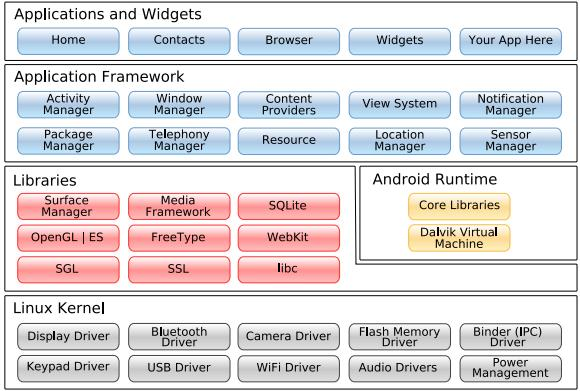
\includegraphics[width=1\linewidth]{images/architecture_android}
\end{center}
\caption{L'architecture de l'Android}
\label{fig:1}
\end{figure}

\subsubsection{L’IDE Android studio}


Android Studio est l’environnement de développement des applications Android officiel de Google qui remplace l’IDE d’Eclipse (avec donc exactement les mêmes fonctionnalités) depuis le 8 décembre 2014, il est basé sur  IntelliJ IDEA. 
Android Studio permet principalement d'éditer les fichiers Java et les fichiers de configuration d'une application Android.

Il propose entre autres des outils pour gérer le développement d'applications multilingues et permet de visualiser la mise en page des écrans sur des écrans de résolutions variées simultanément.
En plus d’être un éditeur de code très puissant, Android Studio offre encore plus de fonctionnalités qui améliorent la productivité des applications Android, tels que :

- Un système de building des applications souple basé sur Gradle.

- Un émulateur rapide et riche en fonctionnalités.

- Un environnement unifié où le développeur peut développer pour tous les appareils
Android.

- L’exécution instantanée (Instant Run) pour apporter des modifications à une appli-
cation en cours d’exécution sans avoir à reconstruire un nouveau APK.

- Modèles de code et une intégration sur GitHub pour construire des fonctionnalités
communes d’applications.

- Des outils et frameworks de tests extensifs.
 
\textbf{Gradle:}


Gradle est un moteur de production qui fonctionne sur la plateforme Java, il est le digne successeur de Maven et de Ant, alliant ces deux outils afin de créer une plateforme de production Java simple à utiliser, et bien adaptée pour les projets Android.
Gradle est intégré à Android Studio et est utilisé afin de gérer et construire les projets Android (en utilisant le langage Groovy).
Il permet entre-autre de gérer la construction d’un projet utilisant plusieurs modules et dépendances de librairies Maven, et ce, de façon très simple.\cite{gradle} 



\subsection{Quelques outils Android utilisés}
\subsubsection{Adapter}

Adapter est un objet permettant de stocker des données provenant des différents sources (contact, rendrez-vous, ...) afin de pouvoir les afficher dans des composants  UI.
les adapters sont donc des interfaces entre les sources de  données et les IHM. 

L'adapter n'est en fait qu'une interface qui définit les comportements généraux des adaptateurs. Cependant, la construction d'un adaptateur, nécessite la dérivation de BaseAdapter.

\begin{figure}[H]
\begin{center}
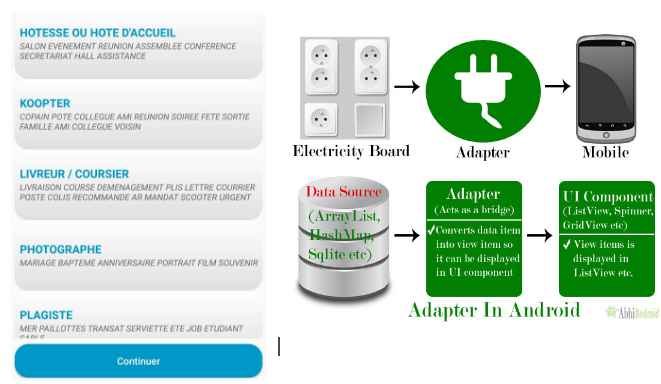
\includegraphics[width=1\linewidth]{images/adapter}
\end{center}
\caption{L'adapter dans l'Android}
\label{fig:2}
\end{figure}


\subsubsection{AsyncTask}


L’AsyncTask permet de réaliser des tâches de manière asynchrone, à la manière de la classe Thread. L’avantage de l’AsyncTask est sa simplicité d’utilisation et d’implémentation. Le Thread secondaire est créé automatiquement et la communication entre les différents Thread est simplifiée.
AsyncTask doit être hérité par la classe qui a été  créé, cette classe doit impérativement implémenter une méthode (doInBackground(Params...)),
Quand un AsynckTask s'exécute il passe par trois étape 


onPreExecute(), appelé sur le thread d’interface avant que la tâche soit exécutée. Cette étape est normalement utilisée pour configurer la tâche, par exemple, en montrant une barre de progression dans l’interface utilisateur.


doInBackground(Params...), invoqué sur le thread en arrière-plan immédiatement après OnPreExecute (). Cette étape est utilisée pour effectuer le calcul de fond qui peut prendre un certain temps. Les paramètres de la tâche asynchrone sont passés à cette étape. Le résultat du calcul doit être retourné par cette étape et sera renvoyé à la dernière étape. Cette étape peut également utiliser publishProgress (Progress …) de publier une ou plusieurs unités de progression. Ces valeurs sont publiées sur le thread d’interface utilisateur, à l’étape onProgressUpdate (Progress …).


onProgressUpdate(Progress...), invoqué sur le thread d’interface utilisateur après un appel à publishProgress (Progress …). Le moment de l’exécution est indéfini. Cette méthode est utilisée pour afficher toute forme de progression dans l’interface utilisateur tandis que le calcul de fond est toujours en cours d’exécution. Par exemple, il peut être utilisé pour animer une barre de progression ou afficher des logs.


onPostExecute(Result), appelé sur le thread UI après la fin du calcul. Le résultat est transmis à cette étape en tant que paramètre.
 
Pour que cette classe fonctionne correctement, il y a quelques règles à respecter :


\begin{itemize}
    \item La classe AsyncTask doit être chargée sur le thread UI. Ceci est fait automatiquement.
    \item L’instance de la tâche doit être créée sur le thread UI.
    \item execute(Param …) doit être invoqué sur le thread UI.
    \item Ne pas appeler OnPreExecute(), onPostExecute (Résultat), doInBackground(Param ...),  onProgressUpdate (Progress ...) manuellement.
    \item La tâche ne peut être exécutée qu’une seule fois (une exception sera levée si une deuxième exécution est tentée).
\end{itemize}\cite{asyncTask} 
 
\subsubsection{ContentProvider}


Un contentProvider sert à stocker et récupérer des données et ainsi les rendre accessibles à toutes les applications. C’est le moyen le plus connu de partager des données entres différentes applications. Par exemple, il existe un Content Provider gérant les Contacts d’un téléphone.
Android propose plusieurs ContentProviders basiques (audio, vidéo, images, informations sur les contacts…). Un contentProvider se compose d’une :

- Uri

- Méthodes (Insert, Update, Delete, Query).


Le chemin d’accès vers un ContentProvider se présente toujours sous forme d’une URI. Par exemple : 

content://com.example.transportationprovider/trains/122

  \textbf{A}      /          \textbf{B}            /    \textbf{C}  /  \textbf{D}  

\textbf{A} : Un préfixe standard, il sert à indiquer que les données sont contrôlées par un ContentProvider.
\newline
\textbf{B} : L’autorité qui contrôle cette URI. Elle identifie le ContentProvider responsable de cette URI. 
\newline
\textbf{C} : Permet au ContentProvider de savoir quelle donnée est requêtée par l’url. Ce segment est optionnel. Un content provider peut exposer plusieurs données (ici les trains) mais on pourrait avoir par exemple les voitures, donc ce ContentProvider pourra gérer deux types de données.
\newline
\textbf{D} : L’id de la donnée qu’on souhaite récupérer. (optionnel)


Pour créer un ContentProvider, il faut : 
    
- Mettre en place un système pour stocker les données (les contents providers utilisent généralement le SQLite).
    
- Étendre la classe ContentProvider.

- Déclarer le Content Provider dans le manifest (AndroidManifest.xml).\cite{provider} 


\subsubsection{SQLite}

 SQLite est une base de données open source, qui supporte les fonctionnalités standards des bases de données relationnelles comme la syntaxe SQL, les transactions et les PreparedStatement. La base de données nécessite peu de mémoire lors de l'exécution (env. 250 ko), ce qui en fait un bon candidat pour être intégré dans d'autres environnements d'exécution.
SQLite est intégrée dans chaque appareil Android. L'utilisation d'une base de données SQLite sous Android ne nécessite pas de configuration ou d'administration de la base de données. 
 
Il faut uniquement définir les instructions SQL pour créer et mettre à jour la base de données. Ensuite, celle-ci est gérée automatiquement, par la plate-forme Android. 
 
L'accès à une base de données SQLite implique l'accès au système de fichiers. Cela peut être lent. Par conséquent, il est recommandé d'effectuer les opérations de base de données de manière asynchrone. 
 
Si l’application crée une base de données, celle-ci est par défaut enregistrée dans le répertoire DATA /data/APP\_NAME/databases/FILENAME. 
 
Ce chemin de fichier est obtenu sur la base des règles suivantes : DATA est le chemin retourné par la méthode Environment.getDataDirectory(), APP\_NAME est le nom de l’application. FILENAME est le nom de la base de données qui est renseigné dans le code de votre application.\cite{sqlite}


\subsubsection{SharedPreferences}

Dans toutes applications, il est souvent nécessaire d'utiliser des variables qui doivent être gardées en mémoire même suite à une fermeture. La solution des Shared Preferences est la plus simple à implémenter.
Les SharedPreferences sont des espaces de stockages propres à chaque application Android. Avec un système de clé;valeur, vous pourrez persister vos données facilement.
Les SharedPreferences sont à récupérer depuis un context, avec context.getSharedPreferences(NAME,MODE).\cite{sharedpreference} 

\subsubsection{Les Logs}

 Comme chacun le sait, la méthode de débogage probablement la plus commune (quelque soit le langage), est d'utiliser des primitives d'affichage sur la sortie standard. Qui ne se rappelle pas des fameux printf du langage C ou des NSLog de l'Objective-C ? Le langage Java offre également la même possibilité grâce à des méthodes de type print du package System.out.
Le développement sur Android ne déroge pas à la règle puisque le SDK fournit une classe nommée android.util.Log qui inclue un bon nombre de méthodes d'aide au développement données dans la liste ci-dessous :\cite{log}

- Log.v : Affiche le message en mode “verbose” c'est à dire “verbeux” ou “abondant” en français.

- Log.d : Affiche le message en mode “debug”, utilisé pour le débuggage.

- Log.e : Affiche le message en mode “error” (erreur).

- Log.w : Affiche le message en mode “warning”, c'est à dire les avertissements.

- Log.i : Affiche le message en mode “info”.


\subsection{Méthodes et technologies déployées}

\subsubsection{Matériel design}

 Lors de la conférence Google I/O 2014, Google a dévoilé le design d'Android Lollipop, design qui portera le nom de Material Design. Ce design met l'accent sur l'unification de l'interface entre les différents types d'appareils : téléphones, tablettes, montres, télévisions mais touche aussi les sites web. De nombreux sites, dont ceux de Google, utilisent le Material Design qui est tout à fait adapté à la pratique du responsive. Pratique qui consiste à adapter l'interface aux dimensions de la fenêtre du navigateur.\cite{materiel}

Le Material Design est apparu quand le Flat Design commençait à faire parler de lui et Google a été rapidement clair sur le sujet : le Material Design n'est pas du Flat Design. Les plus sceptiques sur cette affirmation diront alors que c'est le Flat Design à la Google. Ils n'auront que partiellement raison. Même s'il est vrai que le Material Design partage un visuel similaire au Flat Design, il n'en dispose pas des principes forts du design fait par Google. Les designers de cette entreprise se sont mis au défi de créer un langage visuel pour leur utilisateurs qui se synthétisent en 3 grands principes.

Quelques composants graphiques utilisés dans KOOPT. 

\textbf{Le menu latéral:}
 

Le menu latéral est un composant lié à la navigation. Il se caractérise par un panneau latéral qui se déplace depuis l'extérieur de l'écran jusqu'à un certain niveau à l'intérieur. En général, il se place sur la gauche de l'écran mais il est possible de le placer à droite, voire d'en placer deux, un à gauche et un à droite de l'écran.




\begin{figure}[H]
\begin{center}
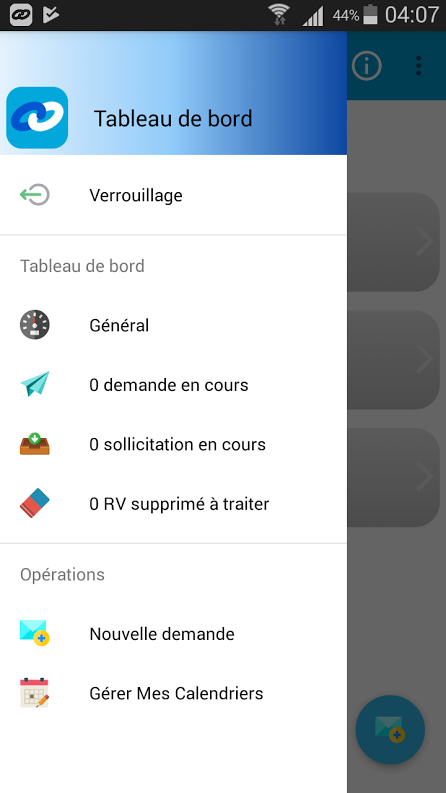
\includegraphics[width=0.5\linewidth]{images/menu_lateral}
\end{center}
\caption{Menu Latéral KOOPT}
\label{fig:3}
\end{figure}




\textbf{Les labels flottants:}
 
 
Ce composant permet à l'utilisateur de saisir du texte dans un espace dédié à cet effet. Par contre, donnez du sens à ce composant était fastidieux. Vous deviez créer un TextView au dessus pour lui donner un titre et y placez un hint.
la bibliothèque de design, nous permet spécifier un label flottant pour votre champ. Ce label se place dans le champ lorsque le curseur n'est pas dessus et se déplace en dehors lorsque vous y placez le curseur.

\begin{figure}[H]
\begin{center}
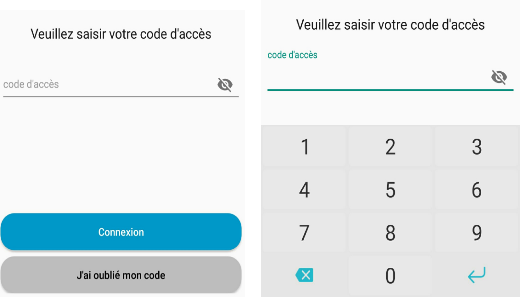
\includegraphics[width=1\linewidth]{images/label_flottant}
\end{center}
\caption{Label flottant KOOPT}
\label{fig:5}
\end{figure}

\subsubsection{Design pattern  Singleton}

KOOPT possède des classes qui doivent être instanciées une seule et unique fois pour cela elle utilise le design pattern Singleton.
le singleton est un patron de conception (design pattern) dont l'objectif est de restreindre l'instanciation d'une classe à un seul objet (ou bien à quelques objets seulement). Il est utilisé lorsqu'on a besoin exactement d'un objet pour coordonner des opérations dans un système. Le modèle est parfois utilisé pour son efficacité, lorsque le système est plus rapide ou occupe moins de mémoire avec peu d'objets qu'avec beaucoup d'objets similaires.
 
pour créer un singleton on doit satisfaire trois composant essentielle :

- Attribut privé et statique qui conservera l'instance unique de la classe.

- Constructeur privé afin d'empêcher la création d'objet depuis l'extérieur de la classe.

- Une méthode statique qui permet d'instancier la classe ou bien de retourner l'unique instance créée.

\begin{figure}[H]
\begin{center}
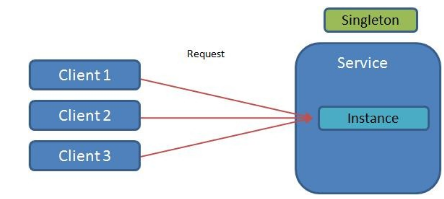
\includegraphics[width=1\linewidth]{images/singleton}
\end{center}
\caption{Singleton}
\label{fig:6}
\end{figure}

\subsubsection{Web service}
 Un service web (ou service de la toile 1) est un protocole d'interface informatique de la famille des technologies web permettant la communication et l'échange de données entre applications et systèmes hétérogènes dans des environnements distribués. Il s'agit donc d'un ensemble de fonctionnalités exposées sur internet ou sur un intranet, par et pour des applications ou machines, sans intervention humaine, de manière synchrone ou asynchrone. Le protocole de communication est défini dans le cadre de la norme SOAP dans la signature du service exposé (WSDL). Actuellement, le protocole de transport est essentiellement HTTP(S).\cite{webservice}


\textbf{Web service REST}

Le World Wide Web est une application conçue selon l'architecture REST. L'architecture du Web remplace donc les concepts applicatifs clients et serveurs par les concepts agents et ressources. Des agents interagissent avec des ressources pour créer, accéder, modifier ou supprimer une ressource. Jusqu'à présent, on parlait surtout de l'interaction entre agents utilisateurs, principalement les navigateurs avec les ressources.

Aujourd'hui, on parle de plus en plus de l'interaction entre agents ressources ; c'est-à-dire la relation entre les ressources : une ressource devient l'agent d'une autre ressource, mais reste elle-même une ressource accessible par d'autres agents. C'est exactement l'architecture décrite par l'exemple d'implémentation applicative des mashups.

Les services web traitent donc d'agents ressources là où le mode opératoire classique du Web parle d'agents utilisateurs. Mais les deux concepts reposent sur la même architecture : REST.
Il n'y a donc pas de différence fondamentale entre l'interaction d'un navigateur avec une ressource et celle d'un Service Web avec une ressource. La principale différence se situe au niveau du format de la représentation des données : HTML pour les navigateurs ou agents utilisateurs, XML ou JSON pour les services web ou agents ressources…

On peut donc définir un service web comme l'implémentation logicielle d'une ressource, identifiée par une URL, et accessible en utilisant les protocoles internet. Les agents s'occupent du contenu, de la représentation de leur état, pas du type de contenu. Il faut donc voir les Services Web comme le moyen de manipuler l'information, et non comme un simple fournisseur de services.


\textbf{TALEND ESB}


L’Enterprise Service Bus, ou ESB, est un ensemble de moyens techniques et organisationnels dont le but est de permettre la communication entre des applications qui, à la base, ne sont pas pensées pour fonctionner ensemble.
 On peut considérer l’ESB comme une nouvelle génération d’EAI (Enterprise Application Integration). La différence majeure avec l’EAI réside dans le fait que l’ESB propose une architecture distribuée décentralisée grâce à l’orchestration de services. Ceux-ci contiennent la logique d’intégration et peuvent être déposés au plus près des applications sources si nécessaire.
Le studio de Talend Open Studio for ESB s’appuie sur le studio de la plateforme unifiée de Talend. Il s’agit donc du même studio, basé sur Eclipse, avec des composants dédiés aux fonctionnalités ESB permettant de gérer la gestion des messages, les services Web, le routage et la transformation des données. Il permet ainsi de développer et de publier des services Web Java, des applications REST et des routes de médiation afin de faire communiquer les applications entre elles.\cite{webservice}
 
\begin{figure}[H]
\begin{center}
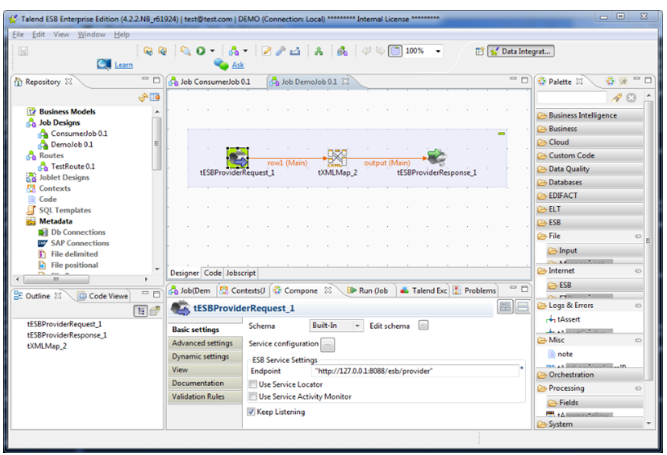
\includegraphics[width=1\linewidth]{images/talend}
\end{center}
\caption{Talend Open Studio for ESB}
\label{fig:7}
\end{figure}

\subsubsection{Crashlytics Fabric}

Crashlytics c’est un outil qui permet de suivre les crashs rencontrés. Concrètement, si une application plante sur l’appareil d’un utilisateur, Crashlytics donne la possibilité d’avoir une trace de ce crash, avec diverses informations comme le nom du téléphone, la version du système d’exploitation, la RAM de libre, l’espace de stockage restant etc. autant d’informations qui peuvent vous aider à cerner la source du problème.

Le dashboard proposé permet de visualiser les crashs par version de l’app, de visualiser le nombre de fois qu’un bug a été rencontré etc.

Cet outil  permet, entre autres, de faire remonter :

- des crashs

- des exceptions

- des messages

- des « customs keys » (pour par exemple connaître l’état de certaines variables)

- des informations sur votre utilisateur.


Renseignez le maximum d’informations permettant de pouvoir cerner la source du problème. \cite{crashlytics} 

\begin{figure}[H]
\begin{center}
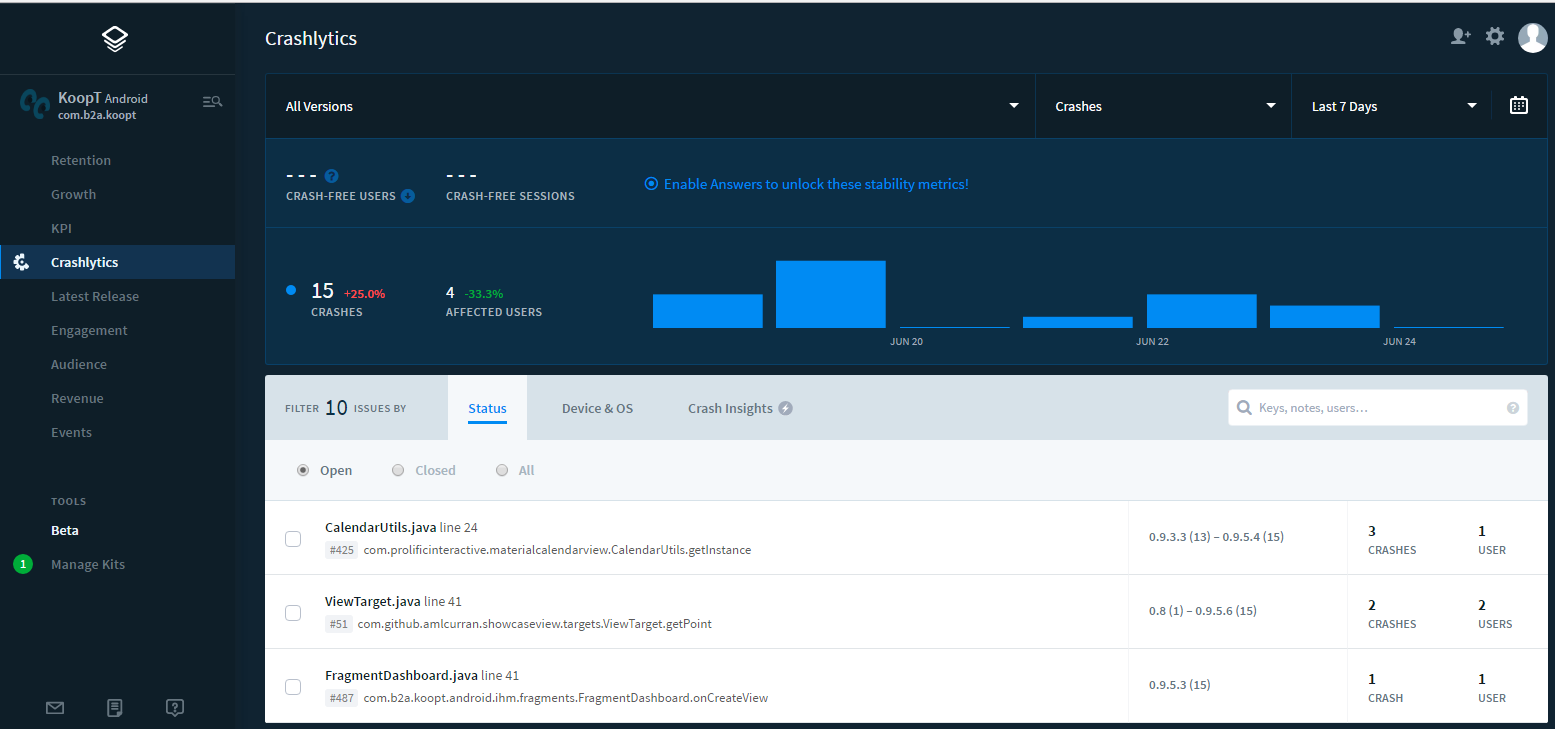
\includegraphics[width=1\linewidth]{images/crashlytics}
\end{center}
\caption{Crashlytics KOOPT}
\end{figure}

\section{Analyse décisionnelle des systèmes complexes}

\subsection{Modélisation des systèmes Complexes}

B-ADSc : "Bucki – Analyse décisionnelle des Systèmes complexes" est une méthode dédiée à la conception et à l’analyse des systèmes et des organisations. Elle se distingue par la prise en compte effective des opérateurs humains avec leurs autonomies, leurs politiques de production, leurs procédés de prise de décision, leur retour d’expérience...

Dans la conception du Système d'Information, les flux des données et des traitements sont soumis aux flux des décisions : en cela B-ADSc généralise les analyses fonctionnelles. Ainsi, le Système d’information est intimement lié à l’Organisation des acteurs (hommes, machines) jusqu'à se confondre.

Conçue dans les années 1990 par Janusz Bucki, docteur en mathématiques et ingénieur automaticien, alors qu’il conduisait des réalisations dans le domaine de l’industrie et de la défense en particulier pour la conception des systèmes à risque et à Intelligence distribuée, cette approche s’est étendue depuis au tertiaire, au monde de l'Internet - Internet des objets - et donne lieu à un enseignement.

Selon cette approche systémique, la caractéristique la plus importante de toute organisation est sa capacité à élaborer des Décisions relatives au pilotage des processus : elle s'attache donc à modéliser et à analyser les organisations selon l'ordonnancement des Décisions et non selon l'agencement des Fonctions...

Pour B-ADSc, une organisation correspond à une hiérarchie opérationnelle d’activités dans laquelle chaque activité représente un «centre élémentaire de prise de décision» pouvant être piloté par un homme ou par une machine.\cite{badsc} 

\begin{figure}[H]
\begin{center}
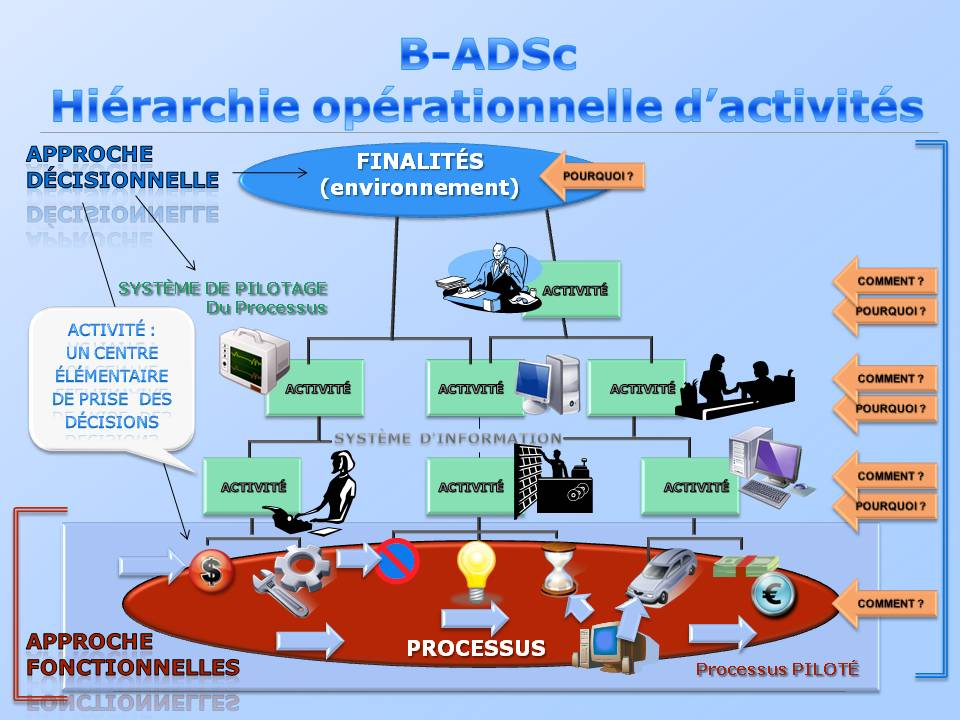
\includegraphics[width=1\linewidth]{images/badsc}
\end{center}
\caption{Hiérarchie opérationnelle d'activités}
\label{fig:8}
\end{figure}


\subsection{ Le concept d’activité}

En Analyse fonctionnelle, l’accent est mis sur les données (schémas de données) et leur transformation ou traitement (schémas des traitements). Ainsi, l’objectif de l’analyste serait plutôt de mettre en exergue le « comment » du système (voir schéma ci-dessous) et pas forcément le « pourquoi de ce comment ».

\begin{figure}[H]
\begin{center}
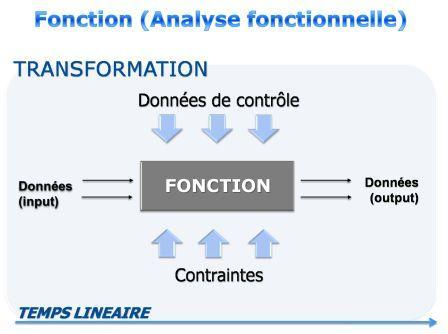
\includegraphics[width=0.5\linewidth]{images/analyse_fonctionnelle}
\end{center}
\caption{L'analyse fonctionnelle}
\label{fig:9}
\end{figure}

Ici, la fonction est comparable à une boîte noire. Elle peut être décomposée en sous-boîtes noires, l'organisation de ces boîtes n'ayant pas pour but de refléter l'organisation des acteurs. En automatisation, la notion de boucle de régulation permet d’adjoindre un « retour » (ou feedback) afin de passer du traitement à la régulation. La fonction peut donc, selon l’évolution du processus, être régulée.

B-ADSc positionne systématiquement le "Comment" dans le contexte de son "Pourquoi" et fait passer du "traitement des données" au "pilotage/régulation des situations" : piloter/gérer un processus signifie décider et contrôler son évolution afin de l’amener à une situation concordant avec les objectifs poursuivis.
La compréhension et l'interprétation des évolutions du processus s’opèrent dans le contexte des buts du décideur, exemple:
Evolution du processus : "je suis chez moi et il commence à pleuvoir"...
si mon but initial est d’arroser le jardin alors - c’est bon – "la nature s’en charge"si mon but est d’aller au théâtre alors - c’est mauvais - "risque d’être mouillé".

Les objectifs et le processus évoluant, le pilotage doit être perpétuellement réadapté : les écarts entre objectifs et réalité doivent diminuer ou, à minima, s’inscrire dans un seuil de tolérance (qui permet d’amener la situation – le processus – au plus près des objectifs poursuivis).
B-ADSc place ici l'activité à l’intersection de deux boucles de régulation qui prennent en compte l’évolution du processus (le comment) et celle des objectifs (le pourquoi).
 
 \begin{figure}[H]
\begin{center}
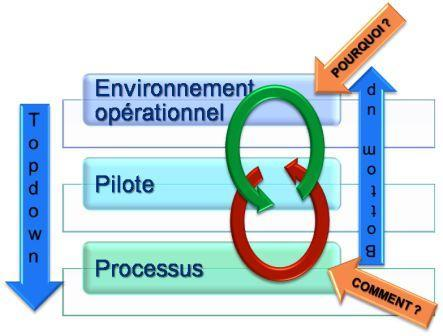
\includegraphics[width=0.5\linewidth]{images/comment_pourquoi}
\end{center}
\caption{L'intersection des deux boucles de régulation le comment et le pourquoi}
\label{fig:10}
\end{figure}
La « brique » de base de B-ADSc est une Activité. Elle est régulée (ou pilotée) par les activités de niveau supérieur qui lui délèguent des objectifs et régule (ou pilote) les activités de niveau inférieur qui constituent son processus.
Ainsi, elle encapsule deux fonctions
(voir schéma ci-dessous):

• « Fd » pour « Fonction décision » 

• « Fe » pour « Fonction évaluation » 

Une activité dispose nécessairement de quatre mémoires distinctes :

1.La mémoire des objectifs assignés par le niveau opérationnel supérieur 

2.La mémoire de l'état du processus piloté 

3.La mémoire des buts des décisions prises par l’activité 

4.La mémoire des changements d’état du processus

 
 \begin{figure}[H]
\begin{center}
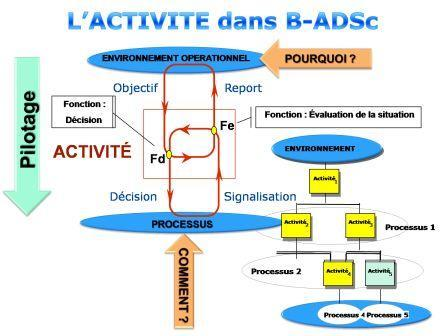
\includegraphics[width=1\linewidth]{images/activite}
\end{center}
\caption{L'activité dans B-ADSc}
\label{fig:11}
\end{figure}

 
B-ADSc interprète systématiquement le comportement d’une activité – prise des décisions, évaluation du processus - dans le contexte des objectifs poursuivis :
Je suis chez moi (« Je » = activité) et il pleut dehors (le « comment » du processus).

• Si mon but initial est d’arroser le jardin alors « c’est bon pour moi » (la nature fera à ma place, je n'ai rien à décider sauf annuler l'arrosage) 

• Si mon but est d’aller au théâtre alors « c’est mauvais pour moi » (je risque d’y arriver mouillé, je décide donc d'annuler ou de prendre un parapluie).\cite{badsc} 


\subsubsection{Caractéristique}

La tolérance et la sensibilité font partie des caractéristiques comportementales d’une activité pilotée.
 
- Tolérance : exprime l’écart maximum admissible pour l'activité pilotée entre l'état perçu du
processus (état interne) et l'objectif poursuivi (objectif externe).
 
- Sensibilité : correspond aux évolutions du processus jugées significatives dans le contexte de
l’un des buts (objectifs internes) de l’activité.
 
Tolérance et sensibilité, peuvent être :
 
• prescrites : imposées de façon structurelle

• conjoncturelles : corrigées (consciemment ou inconsciemment) par le pilote de l’activité
 
Lorsque les objectifs sont validés par le niveau opérationnel supérieur et que les procédures de mise en œuvre des savoirs sont imposées, l’autonomie d’une activité ou d’un acteur et, par là même, sa politique locale de production ou de pilotage ne pourront s’exprimer qu’à travers la tolérance et la sensibilité conjoncturelle.
 
Dans une activité de 1e catégorie il s'agit de la seule forme d’expression de son autonomie.
Dans une activité de 2e catégorie, la politique locale intègre en plus l’expression des préférences
face aux sollicitations simultanées – Fp.
Dans une activité de 3e catégorie, la politique locale comprendra en plus les conditions d’auto
validation des objectifs (externes). \cite{activite}

\subsection{Avantage}

La délégation des décisions, selon la méthode B-ADSc, est par excellence le facteur structurant des organisations. Les délégations conduisent à l’émergence d'activités nouvelles pilotées par des hommes ou par des machines, chacune d’elles constituant un centre autonome de prise des décisions. Pour être efficaces, de telles délégations doivent s’accompagner de la délégation des contrôles correspondants. 

Le rôle de l’activité « déléguant » évolue pour devenir tributaire de décisions de portée plus générale. Suite à une délégation, le nombre de décisions à prendre dans une organisation augmente globalement, tout comme l’effort à fournir pour leur élaboration.
La délégation des décisions peut aussi bien être liée à la création d'activités nouvelles et à l'extension du système d’information.
Compte tenu du coût qui en résulte, toute nouvelle délégation requiert pour sa validation une analyse de la valeur.

Cette analyse, conduite pour évaluer les gains potentiels, suit trois axes :

• amélioration du fonctionnement 
  - décisions plus pertinentes élaborées au niveau du système de délégation : suppression d’une non qualité, 
  
• augmentation de la productivité 
  - par une diminution du délai de prise de décision par rapport au rythme de déroulement du processus : davantage de volumes traités, 
  
• disponibilité accrue des acteurs opérant dans les couches supérieures 
  - grâce à la substitution des décisions déléguées par des décisions plus globales et moins fréquentes: dégageant un potentiel pouvant être réemployé par ailleurs. \cite{badsc}
 
\subsection{Utilisations}

 B-ADSc s'applique à :

- La Conception et l'Analyse des Systèmes et des Organisations	

- La Démarche qualité, la mise en oeuvre des politiques de veille et innovation

- L'Urbanisation en informatique 

- L'Ingénierie des connaissances (gestion des connaissances) et Gestion du retour d’expérience 

- La Conception des Systèmes d’automatisation et des Systèmes Informatiques 

- L'Explicitation des politiques de production et construction de la "convergence des buts" au sein des organisations

- La Robotique 

- Les Systèmes à Intelligence distribuée ou répartie, les Systèmes experts 1 - notamment pour l'Internet des Objets

- Plus généralement : tout Système critique (transports, aviation, systèmes embarqués, …) 
 
 
\textbf{Thin-Track}, moteur évolutif de gestion des actifs ou objets en environnements industriels ou logistiques changeants et incertains, est la réalisation la plus récente de l'utilisation de B-ADSc, tant en conception logicielle qu'en gestion de projet. \cite{badsc}

\subsection{Modélisation des processus dans KOOPT}

Pourquoi la modélisation des processus dans les projets d'organisation ?
pour administrer les processus et les optimiser : 

    • optimiser les coûts internes,
    
    • améliorer sa réactivité et sa rapidité,
    
    • capitaliser ses propres savoirs et expériences,
    
    • identifier et valider les besoins en information de chaque acteur et chaque activité,
    
    • évaluer les opportunités en délégation/automatisation,
    
    • séparer et structurer les rôles et les responsabilités de chacun des acteurs, homme ou machine,
    
    • concevoir les solutions informatisées s'inscrivant naturellement dans la continuité des chaînes
      décisionnelles propres à l’organisation qui les intègre,
    
    • former les nouveaux arrivants,
    
    • gérer efficacement les adaptations aux nouvelles exigences et aux évolutions du contexte opérationnel.
     
     
pour représenter le processus tel qu'il est vécu et tel qu'il évolue : 
Cette nécessaire modélisation des processus implique une mise en évidence de l'organisation réelle.
Il s'agit non de décrire le processus tel qu'il est défini, mais tel qu'il est réellement vécu.
La modélisation sera donc jugée par sa clarté et sa cohérence dans l’explicitation :

    • des objectifs poursuivis à chaque niveau opérationnel,
    
    • des procédés associés à ces objectifs, donc des ordonnancements des décisions,
    
    • de l'utilité des ressources sollicitées durant la mise en œuvre de ces procédés.

\subsubsection{DOMIS}


La modélisation du KOOPT est réalisée par l’outil : DOMIS
DoMIS permet de documenter les processus dans une entreprise ou dans une administration, quelle que soit leur nature.

Il propose un langage générique fondé sur une vision renouvelée de l’organisation.
Une organisation correspond ici à une hiérarchie opérationnelle d’activités dans laquelle chaque activité représente un « centre élémentaire de prise des décisions » pouvant être piloté par un homme ou une machine.
DoMIS à vocation à modéliser les processus par la mise en évidence du système réel de délégation propre à l'organisation. 

Par différence avec les approches classiques et une analyse statique du déroulement des processus – fonctions, 
DoMIS propose une analyse dynamique du système de pilotage et de ses capacités à décider et agir.
L’expression du pilotage sous forme d’ordonnancement des décisions prévaut ici sur la description du déroulement de la fonction :

• « comment nous le faisons » plutôt que « comment ça doit se faire ».

• DoMIS facilite l'identification d'indicateurs internes de gestion plus opérationnels que ceux quantifiant 
simplement les résultats intermédiaires ou finaux. \cite{domis}



%%% Local Variables: 
%%% mode: latex
%%% TeX-master: "isae-report-template"
%%% End: 
\chapter{Etude préalable de projet et implémentation}
\label{sec:etude préalable de projet et implémentation}

\section{Présentation de KOOPT}
Koopt est une application android qui permet de faciliter la vie quotidienne des gens ou chaque personne peut prendre un rendez-vous avec son médecin, coiffeur, etc il permet même d'organiser des sorties entre amis.
toutes personne qui possède un compte koopt est dit koopter. un koopter peut etre demandeur ou receveur de sollicitation ou les deux en même temps par exemple un médecin koopter peut recevoir des sollicitation d’autres koopters (patients) comme il peut solliciter par exemple son coiffeur pour un rendez-vous,  ses amis pour une soiree, une fete ect…
 
Koopt fonctionne sur mobile, en pair-à-pair (pas de serveurs centraux), et permet :

Des services collaboratifs et performants de conciergerie… 

• L’identification en temps réel d’un ou plusieurs acteurs / ressources de confiance pouvant répondre à un besoin, via une cooptation (bouche-à-oreilles) digitalisée ; 

• Pour tout acteur ou ressource, de proposer ses services à la communauté, partager/louer ses biens ; 

• Recommander, dans son réseau, et de proche-en-proche, un offreur de services pour la qualité de ses prestations ;  
 
Des services inédits et innovants de secrétariat…

• L’organisation automatisée et personnelle de chaque agenda des acteurs, permettant leur rencontre dans le temps et l’espace ; 
 
 L’utilisation de ces fonctionnalités dans le cadre des organisations internes des entreprises privées.


\section{L’objectif de KOOPT}

Koopt permet à tout le monde de s’organiser avec tout le monde : famille, voisins, bénévoles, amis, collègues, prestataires… C’est un outil collaboratif de conciergerie et de secrétariat, entièrement automatisé, qui généralise les échanges de ‘gré à gré’. Tout en sécurisant les données personnelles, Koopt simplifie l’organisation de chacun, en permettant :

- De rechercher des partenaires, prestataires, biens… et réserver un créneau disponible en commun; 

- De planifier un nombre important de tâches ou de RDV, de manière automatisée ; dans le respect des objectifs, priorités et contraintes de chacun;  

- De gagner en productivité : plus besoin de consulter une ressource centralisée, un tiers ou d'effectuer des envois multiples de mails pour connaître les disponibilités de chacun; 

- D’assurer ou compléter un revenu, notamment pour les auto-entrepreneurs, artisans, professions libérales, étudiants.

\section{Concurrence - Valeur Ajoutée}

 - La prise de rendez-vous : Les concurrents sont : Gong, Doodle, Calendly, Julie Desk... Toutefois Koopt est la seule application dont l’intelligence est sur le seul Smartphone, et permet de gérer simultanément plusieurs négociations de RDV tout en prenant en compte, en temps réel, les contraintes ou mises-à-jour de calendriers de chacun. C’est aussi la seule à ne partager aucune donnée (protégeant ainsi la vie privée de l’utilisateur). Enfin, Koopt n’est ni une application bureautique nécessitant l’analyse sémantique d’emails, ni un système de sondages en ligne.
 
 - La recherche de partenaires (services, prestataires, ressources...) : de nombreuses applications existent pour des offres ou échanges de services (youpijob, le bon coin, bla-bla car, Jam...), mais sont, soit très spécialisées, soit peu automatisées. Toutes proposent un système de recommandation central, qui ne prend pas en compte les critères subjectifs de chaque utilisateur. Koopt, quant à elle, permet aux utilisateurs d’accéder à différents services en même temps, sans partage de données, selon un système de recommandation de type bouche-à-oreille, et permettant des coûts d’infrastructures plus faibles (serveurs).					
 
KOOPT est la seule intelligence artificielle décisionnelle distribuée, qui fonctionne de manière proactive et intuitive. 




\chapter{Planification et gestion de projet}
\label{sec:Planification et gestion de projet}

\section*{Introduction}

La planification et la gestion de projet au sein de GLOOKAL pour l’application KoopT a été basé sur deux  principaux outils JIRA et SVN.
tout au long du stage on suivaient l’organisation suivante :

- Faire un Update (SVN) au début de chaque journée 

- Faire un Commit (SVN) en fin de chaque journée ou dès qu’une tâche est aboutie avec un message qui contient le numéro de la tâche en cours dans JIRA

- Les tâches à réaliser sont sous forme des fiches JIRA qui porte le nom du rapporteur (Maître de stage) et le nom du responsable ( la personne chargé de réaliser la tâche)

- Ajouter un journal de travail dans JIRA on décrivant le déroulement et le travail réalisé  pour le développement de la tâche ainsi que le temps consacré à sa réalisation.

- Changer le statut de la fiche JIRA de "En cours" à "A valider" une fois la tâche est aboutie.

\addcontentsline{toc}{section}{Introduction.}


\section{JIRA ATLASSIAN}

Jira est un système de suivi de bugs, un système de gestion des incidents, et un système de gestion de projets développé par Atlassian.
Jira est un gestionnaire des demandes, une demande peut être un bug, une anomalie, un incident, une demande d’intervention…  JIRA est un outil de suivi d’activités.
JIRA permet la Planification des projets en créant des user stories et des tickets, en planifiant des sprints et en affectant les à l’ensemble de l’équipe de développement.
 
 
Les demandes ou les tâches KoopT sont gérées à travers quatre status principaux : 

- A Faire : contient les tâches KoopT planifiées à faire prochainement.

- En Cours :  contient les tâches KoopT en cours de développement.

- A Valider : contient les tâches KoopT qui sont abouties mais pas encore validées.

- Résolues : contient les tâches KoopT abouties et validées. 

\section{Subversion (SVN)}

Subversion (en abrégé svn) est un logiciel de gestion de versions, distribué sous licence Apache et BSD. Il a été conçu pour remplacer CVS. Ses auteurs s'appuient volontairement sur les mêmes concepts (notamment sur le principe du dépôt centralisé et unique) et considèrent que le modèle de CVS est bon, seule son implémentation est perfectible.

Subversion fonctionne donc sur le mode client-serveur, avec :

- un serveur informatique centralisé et unique où se situent :
les fichiers constituant la référence (le « dépôt » ou « référentiel », ou « repository » en anglais),
un logiciel serveur Subversion tournant en « tâche de fond » ;

- des postes clients sur lesquels se trouvent :
les fichiers recopiés depuis le serveur, éventuellement modifiés localement depuis,
un logiciel client, sous forme d'exécutable standalone (ex. : SmartSVN) ou de plug-in (ex. : TortoiseSVN, Eclipse Subversive) permettant la synchronisation, manuelle et/ou automatisée, entre chaque client et le serveur de référence
 

\chapter{Compatibilité sous Android}
\label{sec:Compatibilité sous Android}

\section*{Introduction}

Toutes les icônes et les images de l’application KOOPT sont créées sous forme d'images vectorielles qui sont compatibles qu’avec les versions Android supérieure ou égale à 5.0 et qui ne sont pas compatibles avec les versions inférieures.
Ma mission était de gérer la compatibilité de KOOPT avec toutes les versions Android, pour cela on a ajouté des wrappers pour les images vectorielles pour qu’elles puissent être affichées sur tous les smartphones Android sur n’importe qu’elle version.

\addcontentsline{toc}{section}{Introduction.}

\section{Images Vectorielles}

L’ajout d’images à un projet android se fait via les drawables. Pour des raisons de performance, en fonction de la taille de l’écran nous devons fournir une image possédant une plus ou moins grand résolution. C’est pour cela qu’une même image sera ajoutée dans plusieurs tailles dans les dossiers mdpi, hdpi, xhdpi, etc. Ce qui augmente rapidement le poids de l’application.
Cette contrainte est souvent mal perçue par les développeurs, car elle demande un effort supplémentaire entre l’export de la maquette et l’ajout au projet, et souvent se solde par l’ajout d’images de mauvaise résolution ou d’une seule image dans les drawable.
 
C’est pour cela il existe un type d’image résistant à la résolution, c’est à dire pouvant être affichées sans perte de qualité peut importe la résolution à laquelle seront affichées, elles sont appelées images vectorielles.

Elles ne sont pas composées de pixel contrairement aux png ou jpeg, mais de définitions de formes, associées à des couleurs. Ce qui a pour résultat de re-calculer la forme lorsque l’on change la résolution de l’image au lieu de rasteriser celle-ci.

Depuis android 5.0, il est maintenant possible d’utiliser ces images dans les projets, en utilisant les vector drawables.
Pour créer une image vectorielle, il suffit d’écrire les détails de la forme au sein d’une balise <vector> dans un fichier drawable xml.\cite{imagevectorielle}

\section{Solution des Wrapper}

Les Wrapper sont des fichiers XML qui encapsulent les images vectorielles afin qu’elles puissent être compatibles avec toutes les versions android; c’est la technique qu’on a adapté pour la problématique de compatibilité en évitant d’ajouter les images en  plusieurs tailles dans les différents  dossiers Drawable  mdpi, hdpi, xhdpi, etc.
 

\chapter{Amélioration technique de KOOPT}
\label{sec:Amélioration technique de KOOPT}

\section*{Introduction}


Ce Chapitre présente les missions qui me sont confiées au niveau de l’amélioration technique de KOOPT et qui consiste l'évolution de certains IHM de l’application ainsi que le développement des sous-fonctionnalités de KOOPT.
\addcontentsline{toc}{section}{Introduction.}


\section{L’utilisation de KOOPT}

\subsection{Les écrans d’aide KOOPT}
Afin de faciliter l’utilisation de KOOPT pour les utilisateurs et de les guider sur le fonctionnement général de KOOPT, on a mis en place des écrans d’aide pour toute l’application, accessibles dans toutes les IHM de KOOPT.
Pour cela, on a utilisé la librairie ShowCaseView.

\subsection{ShowCaseView}
La bibliothèque ShowcaseView (SCV) est conçue pour mettre en évidence des parties spécifiques d'applications à l'utilisateur avec une superposition distinctive et attrayante. Cette bibliothèque est idéale pour indiquer les points d'intérêt pour les utilisateurs, les gestes ou les objets obscurs mais utiles.

 \begin{figure}[H]
\begin{center}
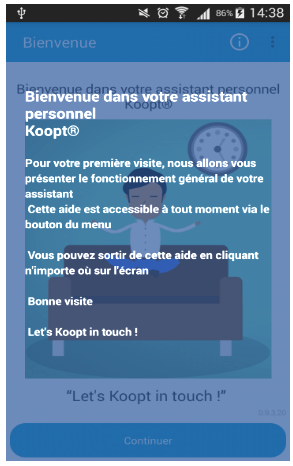
\includegraphics[width=0.5\linewidth]{images/help}
\end{center}
\caption{Écran d'aide de la page d'accueil KOOPT}
\label{fig:12}
\end{figure}
Target: 
 
ShowCaseView fournit la possibilité d’utiliser des targets,  qui sont sous forme de cercles, qui 
mettent  le focus sur un objet spécifique dans un IHM afin de pouvoir aider et guider l’utilisateur sur l’utilisation de cet objet. 

 \begin{figure}[H]
\begin{center}
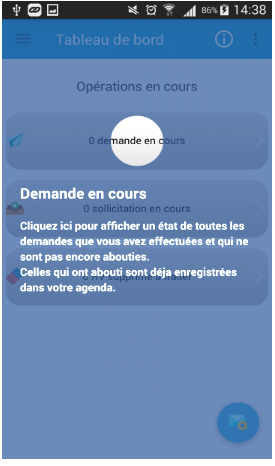
\includegraphics[width=0.5\linewidth]{images/helptarget}
\end{center}
\caption{Écran d'aide du Tableau de bord KOOPT}
\label{fig:13}
\end{figure}

\subsection{Inconvénient}

ShowCaseView offre un support et une aide pour l’utilisateur de l’application à travers la manipulation facile et flexible des Targets.
Le positionnement d'un texte spécifique à une Target est ingérable et produit un écran d’aide mal structuré dans certains cas où l’application est lancée sur des smartphones avec un petit écran.

\section{Alerte des Koopters}
Après une organisation de rendez-vous effectuée par un utilisateur de KOOPT avec d’autres Koopters,  l’application donne la possibilité d’alerter ces derniers s'il n’y a aucune réponse reçue  de leur part. pour cela on a mis en place un système d’envoi de SMS qui permettra aux organisateurs de rendez-vous d’envoyer un SMS d’une façon automatique aux autres Koopters concernés dont l’application KOOPT est désactivée afin de pouvoir la relancer.

 \begin{figure}[H]
\begin{center}
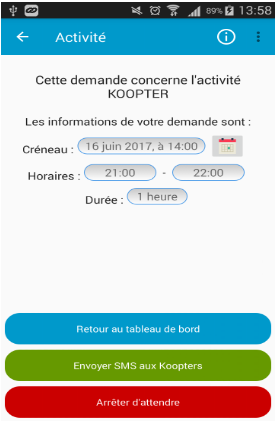
\includegraphics[width=0.5\linewidth]{images/sendsms}
\end{center}
\caption{IHM KOOPT qui permet l'envoi de SMS à un Koopter}
\label{fig:15}
\end{figure}

Pour cela on a utilisé API SMSManager.

\subsection{SMSManager}
SmsManager est la classe qui  gère l’envoi des  SMS dans une application Android . Il n'est pas possible d'avoir une instance de cette classe, mais il faudra utiliser une méthode statique SmsManager.getDefault() pour en récupérer une par défaut.

SmsManager sms = SmsManager.getDefault();

Sécurité : 
Pour envoyer un SMS, il faut d'abord autoriser l'application et ajouter la permission d’envoi des SMS Dans le fichier AndroidManifest.xml de l’application :
<uses-permission android:name="android.permission.SEND\_SMS"/>
\subsection{Contraintes}
Les SMS ont une taille de 160 caractères maximum. Au delà, il sera nécessaire de découper le texte en bloc de 160 caractères et de les envoyer les uns après les autres.
Dans KOOPT on a choisi un message réduit qui ne dépasse pas 160 caractères et qui contient toutes les informations nécessaires pour alerter les Koopters.

\section{Contact pour nouvelle activité}

KOOPT donne la possibilité à ses utilisateurs de suggérer de nouvelles activités mais pas d’une façon automatique pour des raisons de control de l’application. pour cela, on a implémenté un mécanisme de contact avec l’administrateur de KOOPT par Email dans lequel l’utilisateur propose l’activité qu’il souhaiterait ajouter à la liste des activités déjà existantes KOOPT.

 \begin{figure}[H]
\begin{center}
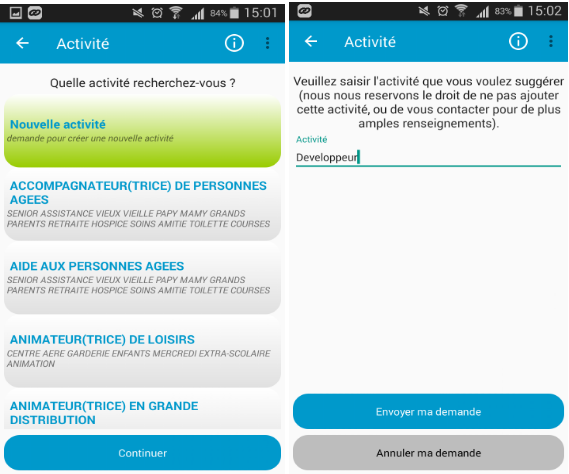
\includegraphics[width=1\linewidth]{images/newactivite}
\end{center}
\caption{Suggestion d'ajout d'une nouvelle activité à KOOPT}
\label{fig:16}
\end{figure}


 \begin{figure}[H]
\begin{center}
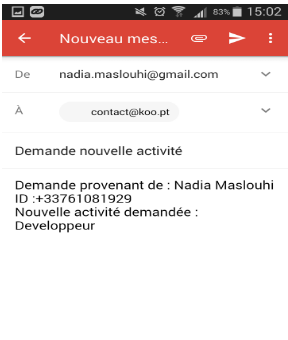
\includegraphics[width=0.5\linewidth]{images/sendmail}
\end{center}
\caption{Envoi d'Email au directeur de KOOPT}
\label{fig:17}
\end{figure}

Après la saisie de l’activité souhaitée, l’utilisateur clique sur "Envoyer la demande". L’application Email du smartphone s'ouvre avec un Email prés-rempli. l'utilisateur n'as plus qu'a cliquer sur le bouton qui renvoyait l'Email.
L'administrateur KOOPT traite les demandes reçues, et ajoute les activités par une application dédiée. 
\subsection{Inconvenient}
L’envoi d’un Email automatique reste toujours un obstacle pour KOOPT et aussi pour d’autres applications car la programmation et la configuration d’un tel mécanisme nécessite la récupération des identifiants qui sont propre à l’utilisateur (Email et mot de passe) pour pouvoir s’authentifier et envoyer un Email directement sans passer par des applications intermédiaires d'Email.

Pour cela dans KOOPT on était censé de donner le choix à l’utilisateur pour sélectionner l’application avec laquelle il veut envoyer son Email (Exemple : Gmail).


\section{Gestion des notifications }
KOOPT s’appuie beaucoup sur les notifications lors de son utilisation.
en lançant KOOPT une notification KOOPT apparaît sur le smartphone et qui reste persistante sauf si l’utilisateur a quitté KOOPT, En cliquant sur cette dernière, l’application se lancera de nouveau.

KOOPT utilise aussi les notifications pour alerter l’utilisateur dans plusieurs cas (Réception d’une sollicitation , Réception d’une confirmation de rendez-vous …). 
Toutes ces notifications nécessitent une gestion pour éviter les notifications obsolètes, c’est à dire le cas où l’utilisateur a toujours une notification pour ouvrir un IHM spécifique qu’il a déjà ouvert. 

Donc on a implémenté un mécanisme qui teste à chaque apparition d’une notification si l’IHM demandée a déjà été ouverte par l’utilisateur. dans ce cas la notification sera supprimée automatiquement en utilisant le NotificationManager.
\subsection{Notification Manager}
Pour envoyer des notifications, il faut passer par  l'instance du service de notifications d'Android (Notification Manager). Il s'agit d'un service gérant pour toutes les applications ces notifications. Celui-ci va trier ces notifications par ordre de priorité (qui correspond au paramètre notification when précisant quand la notification a été envoyée) pour en informer ensuite l'utilisateur.\cite{notification}
 
Notification Manager permet d’envoyer, modifier et annuler une notification grâce a son identifiant.

\section{Les Settings KOOPT  }

Dans KOOPT, il est nécessaire de garder en mémoire les différentes informations d’un utilisateur (Numéro de téléphone , Code d'accès, nom, adresse, activités …) même suite à une fermeture de l’application. La solution est de créer des Settings (Instance de  SharedPreferences) pour stocker toutes les informations nécessaires afin qu’il puisse les modifier ultérieurement.


\subsection{Changement du Code d’accès KOOPT}

Le code d’accès fait parti des informations qui sont stockées dans les settings de KOOPT et que l’utilisateur a le droit de modifier.
La modification du code d’accès se fait à l’aide du web Service KOOPT\_changePassword qui a pour rôle le changement du mot de passe d’un utilisateur en passant par plusieurs étapes : 

- La vérification de l’ancien code d'accès.

- La génération d’un code de confirmation à 6 chiffres qui sera envoyé à l’utilisateur par un SMS ( Valable 10 minutes).

- La vérification du code de confirmation et du délai de confirmation
 
Le web Service a été développé à travers la plateforme Talend (Talend Open Studio) par des composants dédiés aux fonctionnalités ESB.
 
 \begin{figure}[H]
\begin{center}
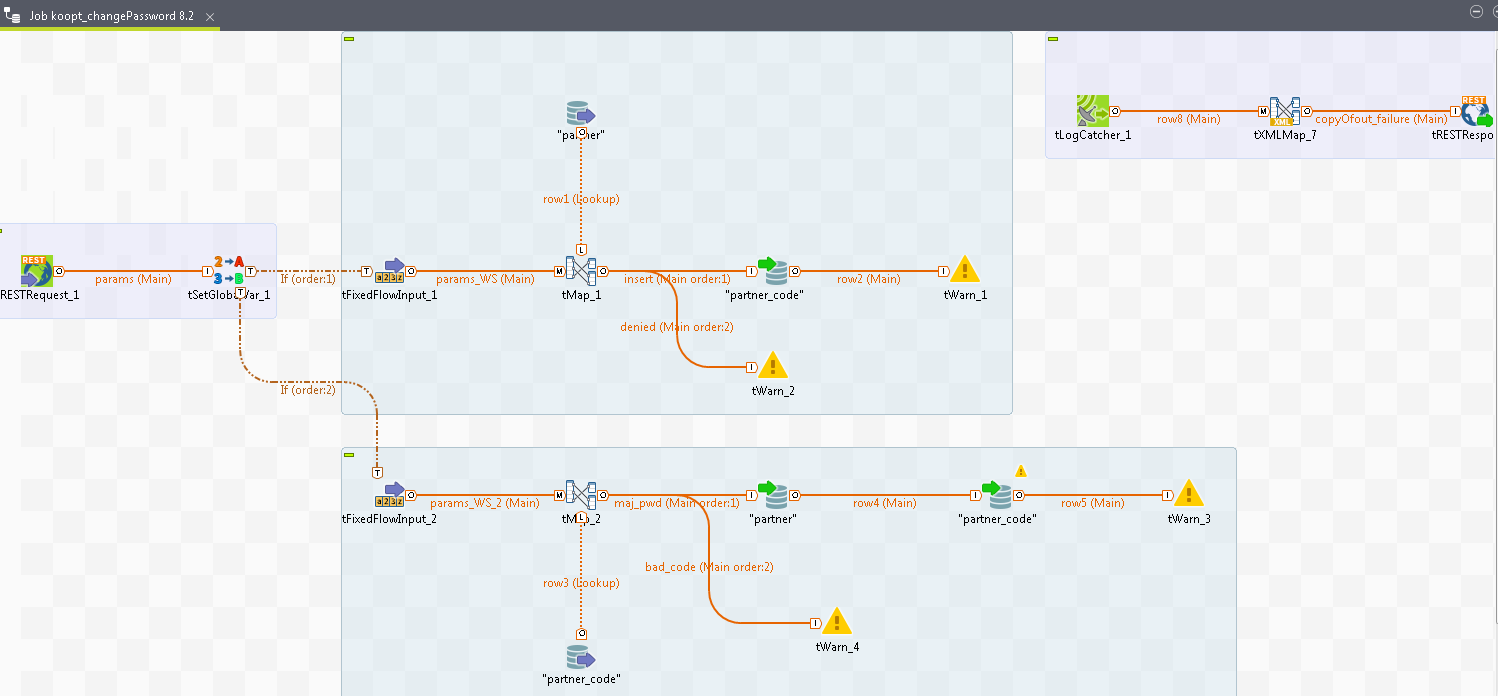
\includegraphics[width=1\linewidth]{images/webservice}
\end{center}
\caption{Web service ChangePassword\_KOOPT}
\label{fig:18}
\end{figure}
 
Le web service renvoie des réponses qui contiennent soit des objets ( code de confirmation généré) ou des messages pour montrer le résultat des vérifications réalisées. 
Suite à ses réponses, on gère la modification du code d'accès, préalablement cryptée, en le modifiant dans les Settings KOOPT.



\chapter{Débogage du Moteur KOOPT }
\label{chap:debogage du Moteur KOOPT }


Après la publication de la version beta de KOOPT pour donner la possibilité aux utilisateurs de tester l’application, on a pu cumuler les différents retours des testeurs,
qui concernent soit des bogues soit d'améliorations UX/UI (fonctionnalités,ergonomie)
  
Pour détecter les sources des différents problèmes, on a utilisé les LogCats pour nous aider à tracer l’exécution de l’émulateur et de l’application.
KOOPT dispose de ses propres Logs qui tracent l’exécution et le comportement de son moteur.
 
  \begin{figure}[H]
\begin{center}
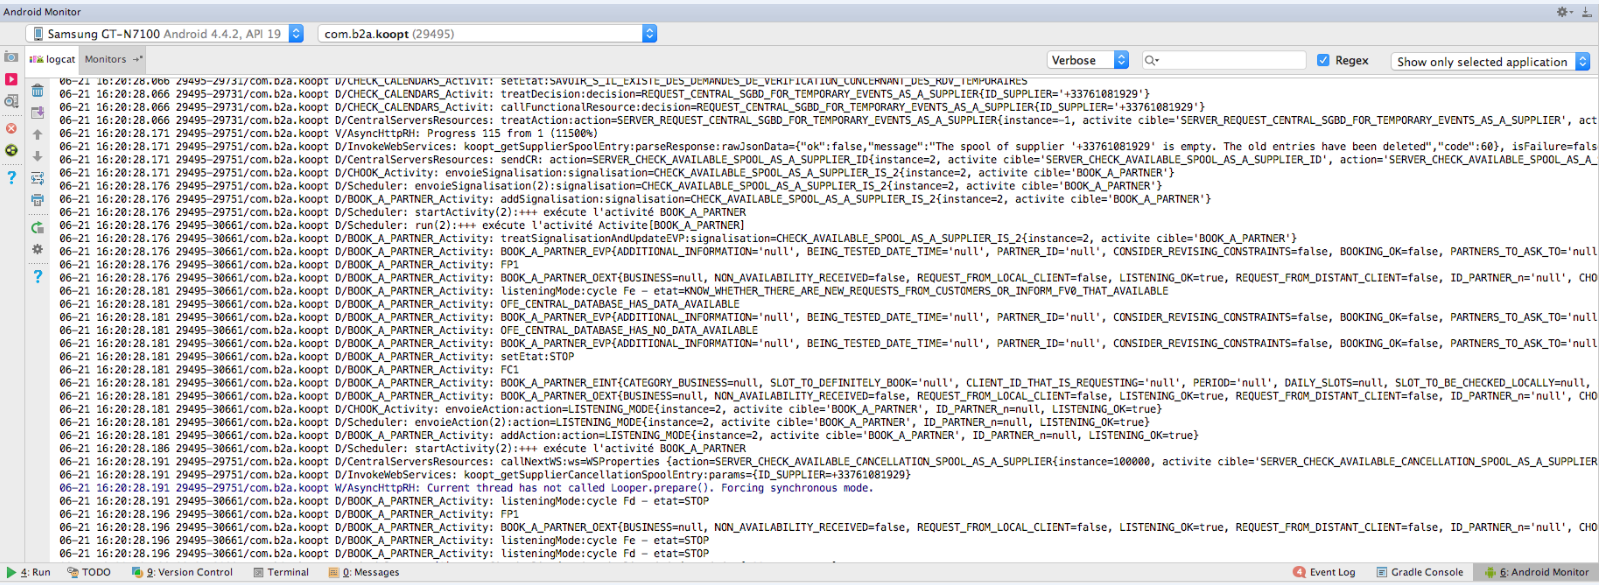
\includegraphics[width=1\linewidth]{images/androidmonitor}
\end{center}
\caption{Android Monitor}
\label{fig:19}
\end{figure}
 
Certains bugs proviennent de la conception de KOOPT, il était donc nécessaire d'interagir avec le responsable de la conception pour bien tracer le comportement du moteur et détecter la source de l’erreur.
 

\chapter*{Conclusion}
\label{chap:conclusion}

Ainsi, j’ai effectué mon stage de  Master 1 MIAGE (Méthodes informatiques appliquées à la gestion des entreprises) au sein de l'entreprise GLOOKAL SAS, qui est une expérience très satisfaisante et enrichissante. Faire partie d’une équipe dynamique, accueillante et compétente, travailler dans d’aussi bonnes conditions et pouvoir mettre en pratique mes connaissances théoriques que j’ai acquis sont autant de choses positives que j’en retire. 
 
Ma mission durant ce stage c’était la contribution aux développement de l’application KOOPT et qui s’étalait sur trois phases. La première phase était la compréhension du concept B-ADSc sur lequel se base la conception de KOOPT ainsi que l’architecture technique de KOOPT, la deuxième phase consistait le développement technique  de l'application, et la dernière c’était le débogage du moteur de KOOPT.
					
Ce projet a également représenté une bonne expérience pour moi au niveau de la programmation mobile (Android). En effet, ces dernières années ont eu une croissance spectaculaire du marché des applications mobiles, et applications Android précisément.
Ainsi cette application arrive comme la conclusion de ma formation sur la programmation mobile android eu au cours de mon cursus en Master 1 MIAGE. 
	
De surcroît ce projet m’ a permis de raffiner mes capacités d’abstraction et de conception en découvrant tout un nouveau concept de modélisation (B-ADSc). Par ailleurs,j’ai tiré grand profit, aussi bien au niveau méthodologique et au niveau technologique.
 
		 	 	 							
De plus il est nécessaire de rappeler qu’à la date de rendu de ce rapport, le stage n’est pas encore terminé, puisqu’il se termine le 31 juillet 2017. Ainsi donc, pendant les mois restant, d’autres améliorations seront apportées a KOOPT auxquelles je vais contribuer.
 
\addcontentsline{toc}{chapter}{Conclusion.}


\appendix

\bibliographystyle{authoryear-fr}
\bibliography{references}


\end{document}